\graphicspath{{ch2_background/}{Figures/}}

\chapter{Background}
\label{chapter:background}

% Sections: 
% Introduction to Machine Learning in Vision
%   Overview of Machine Learning (ML) - This is not necessary as a subsection.
%   Deep Neural Networks (DNN) in Computer Vision
%   Key Concepts in ML for Vision Applications - feature extraction, model architectures (bridge for the next), learning paradigms (introduce only), evaluation metrics, 

% Attention Mechanisms and Vision Transformers
%   Understanding Attention in Neural Networks
%   Vision Transformers (ViT): An Emerging Paradigm -> say also that they are not much better than convnets for medical things
%   Prompts for Vision Transformers - look at ECCV related work section

% A bridge here

% Gaussian Processes
%   Multivariate
%   Regression
%   The example

% Training Strategies in Machine Learning
%   Supervised Learning: The Traditional Approach. 
%       - Formal definition (MLE)
%       - Usage in neural networks, different loss functions
%       - Problems: overfitting, generalization error, data availability (short)
%   Semi-Supervised and Unsupervised Learning: Advanced Techniques
%   Reinforcement Learning and Other Methods - very short

% Domain Adaptation in Computer Vision
%   Why DA is important
%   The amount of information determines the flavor: Types of Domain Adaptation (Unsupervised, source free...)
%   Domain Adaptation in Real-World Applications  ---> Probably not!

% Elements of Ophthalmology
%   Imaging the Retina --> technical stuff on how OCTs work and what we can get. Also fundus
%   Seeing in an OCT --> diseases that can be seen, concept of biomarker
%   Evaluating Vision: The ETDRS Grid --> Just talk about it
%   Merging DL and Ophthalmology --> How and why you would put these two together (a lot of images, difficult to segment...)

% Summary and Conclusion
%   Connection to the rest of the thesis


\sidechaptersummary{Convolutional Neural Networks, Vision Transformers, Gaussian Processes, Deep Learning Training, Domain Adaptation, Elements of Ophthalmology}
\desctotoc{Convolutional Neural Networks --- Vision Transformers --- Gaussian Processes --- Deep Learning Training --- Domain Adaptation --- Elements of Ophthalmology}

\subsubsection{Synopsis} This chapter examines the field of computer vision, with a specific focus on applications in ophthalmology. It begins with an introduction to machine learning in vision, highlighting deep neural networks and other concepts such as feature extraction or evaluation metrics. Next, attention mechanisms and vision transformers are explored, examining their efficacy compared to traditional convolutional networks, particularly in medical imaging. This opens the field to discuss novel training procedures distinct from those traditionally used for convolutional networks. Before looking into training strategies for machine learning, Gaussian processes and regression are briefly overviewed. Then, domain adaptation in computer vision is addressed, explaining its real-world significance and different types. Finally, attention turns to ophthalmology, covering some technical aspects of retinal imaging using optical coherence tomography (OCT), the identification of pathologies through these imaging techniques, and the concept of biological markers. The chapter concludes by discussing the integration of deep learning and ophthalmology.

% This chapter examines the field of computer vision, with a specific focus on applications in ophthalmology. We begin with an introduction to machine learning in vision, highlighting deep neural networks and other concepts such as feature extraction or evaluation metrics. Next, we explore attention mechanisms and vision transformers, examining their efficacy compared to traditional convolutional networks, particularly in medical imaging. This opens the field to discuss novel training procedures distinct from those traditionally used for convolutional networks. Before looking into training strategies for machine learning, we briefly stop to overview Gaussian processes and regression. Then, we address domain adaptation in computer vision, explaining its real-world significance and different types. Finally, we turn our attention to ophthalmology, covering some technical aspects of retinal imaging using optical coherence tomography (OCT), the identification of pathologies through these imaging techniques, and the concept of biological markers. The chapter concludes by discussing the integration of deep learning and ophthalmology.



% Introduction to Machine Learning in Vision
%   Overview of Machine Learning (ML) - This is not necessary as a subsection.
%   Deep Neural Networks (DNN) in Computer Vision
%   Key Concepts in ML for Vision Applications - feature extraction, model architectures (bridge for the next), learning paradigms (introduce only), evaluation metrics, 

\section{Machine Learning in Computer Vision}\label{sec:ml}

The field of computer vision saw its birth during the second half of the twentieth century. Initially, it was regarded as a relatively straightforward problem\sideauthorcite{sejnowski2018deep}, with early efforts focused on the manual extraction of features using algorithms that attempted to emulate the capabilities of the human visual system. However, the realization that features could take an infinite number of forms led to the hard truth that vision was a more complex problem than had been previously assumed. Soon, these manual efforts were redirected towards automatic feature extraction, with machine learning becoming a pivotal component. Since then, machine learning has significantly transformed the field of computer vision, enabling systems to learn from large datasets and make accurate predictions automatically. Deep learning, a subset of machine learning, has driven these advancements, demonstrating exceptional capabilities in tasks such as image recognition, object detection, and scene understanding. 

\subsection{Deep Learning in Computer Vision}
\label{subsec:deep_learning}
At first sight, the term ``Deep learning'' may sound pretentious. Why is it called ``Deep'' and what differentiates it from ``Machine learning''?  As it has been mentioned above, deep learning refers to a subset of techniques within the machine learning paradigm. These techniques have shown such unprecedented capabilities in world understanding that have led to the emergence of a new field. However, what distinguishes them from traditional machine learning algorithms is the use of neural networks with multiple layers. The term ``deep'' alludes to the stacking of these layers.

Neural networks lie, therefore, at the core of deep learning. Formally, these are functions $f$ that transform a set of inputs $\vect{x}$ into a set of outputs $\vect{y}$ making use of their parameters $\vect{\theta}$: 
\begin{equation*}
    \vect{y} = f(\vect{x};\vect{\theta}), f: \real^N \rightarrow \real^M.
\end{equation*}

Thanks to their parameters, they work as universal function approximators\sideauthorcite{cybenko1989approximation}, meaning that with appropriate weights, they can represent a variety of functions. The goal of neural networks is to learn these weights.

The standard deep learning model is the \autoindex{multilayer perceptron} (MLP), or feed-forward neural network\sideauthorcite{rumelhart1986learning}. Here, the previously mentioned function $f$ is composed of several layers to produce an output:
\begin{equation*}
    f(\vect{x}) = f_L(f_{L-1}(...f_1(\vect{x}))).
\end{equation*}

Each layer contains the parameters $\vect{\theta}_l$ as a set of weights $\vect{W}_l$ and biases $\vect{b}_l$ that are applied to the input. Moreover, in order to fulfill the universal approximation theorem, each layer also includes a non-linear transformation or activation function $g_l$. Without a non-linear activation, all the transformations would be affine, and therefore, the resulting function would also be affine. Combining all these parts, the layer function results in:
\begin{equation*}
    f_l(\vect{x};\vect{W}_l,\vect{b}_l) = {g_l}(\vect{W}_l\vect{x} + \vect{b}_l).
\end{equation*}

The activation function can take several forms, and their in-depth characterization lies outside the scope of this thesis. The most used functions are Rectified linear unit (ReLU)\sidecite{nair2010rectified}, sigmoid, or softmax\sidenote{ReLU: $$g(\vect{x})=\max(0, \vect{x}),$$ Sigmoid: $$g(\vect{x})=(1+\exp(-x))^{-1},$$ Softmax: $$g(\vect{x})=\dfrac{\exp(x_i)}{\sum_j\exp(x_j)}, \forall i\in {1,...,J}$$ Note that the softmax activation function acts on all the components of $\vect{x}$ in the layer. Whereas ReLU and sigmoid act individually.}. We instantiate the reader to \yeartextcite{dubey2022activation} for a thorough description and analysis of activation functions.

\textfig[t]{1}{Figures/mlp.pdf}{Multi-layer perceptron with three layers, a two-dimensional input, and a one-dimensional output. Subindices denote the layer number, $h_i$ is the activation function of layer $i$, $\vect{W}$ and $\vect{b}$ are weights and biases, respectively. The color of the arrows represents the variable weight values, which mediate the contribution of a node in the subsequent layer.}{fig:mlp}

The theoretical foundation for a single node (or neuron, hence \textit{neural} networks) allows us to build an MLP, as depicted in \Cref{fig:mlp}. In that figure, we see a multi-layer perceptron with three layers, a two-dimensional input, and a one-dimensional output. All the layers between the input and the output are called \textit{hidden layers}. MLPs have two main features: firstly, all the nodes in one layer are connected to all the nodes in the subsequent layer. Thus, the contribution of each link is mediated by the weight $\vect{W}_l$. Secondly, there are no backward connections\sidenote{The output of layer $i$ does not return to layer $i-1$ in any way.}, hence the name \textit{feed-forward neural networks}.

Multilayer perceptrons have demonstrated remarkable performance on a variety of tasks, which has led to their becoming the fundamental component of deep learning. Nevertheless, their application to computer vision is not straightforward for several reasons. Images are composed of a set of pixels that do not exist independently from each other. The correlation between pixels is stronger when they are in close proximity, as they are more likely to belong to the same object. From \Cref{fig:mlp}, we can see that MLPs take vectors as inputs, but spatial information is lost once an image is transformed into a flattened vector. Moreover, even images that are considered low-resolution contain over 10,000 pixels\sidenote{An image that is 100 pixels in width and height, for example.}, and, as explained above, MLP layers are fully connected. Consequently, the number of parameters grows linearly with the number of nodes. Therefore, computation and storing space turn prohibitively expensive as the neural network grows. On the same line, such high dimensional spaces might suffer from the curse of dimensionality\sidedef{curse of dimensionality}{As the number of dimensions increases, so does the number of configurations. Thus, the amount of information covered by an observation decreases~\cite{bellman1957dynamic}.}, whereby the information supplied by each data point decreases.

\subsubsection{Convolutional Neural Networks (CNNs)} Devised by \yeartextcite{lecun1998gradient}, CNNs are a type of neural network designed for the processing of data with spatial correlation, such as time series (1D) or images (2D). They owe their name to the convolution operation, which represents the fundamental operation of these networks. Convolution is an operation on two functions $x(t)$ and $w(t)$ typically denoted as $(x\ast w)(t)$. It is defined as

\begin{equation}
    (x\ast w)(t)\coloneqq \int x(\tau)w(t-\tau)d\tau,
    \label{eq:convolution}
\end{equation}
where the limits of integration are defined by the support of the functions $x(t)$ and $w(t)$. 

We can now interpret an image as a discrete two-dimensional function of the spatial position $x(i,j): \N^2\rightarrow [0, 255]^3$, whereby each pixel position returns a color intensity in RGB8. In this case, the function $w$ must also be two-dimensional and discrete. Thus, \Cref{eq:convolution} changes to:

\begin{equation}
    (x\ast w)(i,j)\coloneqq \sum_m\sum_n x(m,n) w(i-m, j-n).
    \label{eq:convolution_2d}
\end{equation}

This is the operation performed by convolutional layers in CNNs, where $x$ represents the image and the function $w$ is called \textit{kernel}\sidenote{Or filter. They will be treated as synonyms along this text}. The output is named \textit{feature map}. Usually, the kernel will be smaller than the image, and its parameters will be learned.

From \Cref{eq:convolution_2d}, we notice that opposite to MLPs, convolutional layers only affect the neighbors of the pixel $(i, j)$, favoring spatial relations. Also, for this reason, the number of parameters is significantly lower. Furthermore, the convolutional setup enables the usage of variable size images. 

The output of a two-dimensional convolutional layer is also two-dimensional. In this case, how do we output a single value prediction, as done in \Cref{fig:mlp}? The answer is pooling layers\index{pooling layer}. These layers summarize the features in patches of the feature map, effectively downsampling the feature map by the size of their kernel. The most common pooling operations are average pooling and maximum pooling, which average and take the maximum value of a patch, respectively.

\textfig[t]{0.8}{Figures/cnn_image.pdf}{Illustration of a convolutional layer. The kernel slides over the input image and detects specific patterns, such as edges or textures. The resulting feature map highlights the presence of these patterns across the input image.}{fig:cnn_image}

CNNs are usually not fully convolutional, meaning that after a series of convolutional layers, they contain a global pooling operation that transforms the feature maps into a flattened vector, which can be input to the MLP responsible for the final prediction. In \Cref{chapter:oct}, we will dive deeper into the different ways of performing this operation. 

\subsubsection{Attention Networks}
Attention networks have rapidly become the cornerstone for large models due to their impressive performance and generalization capabilities. They are composed of MLPs whose results are combined in a distinct manner from the feedforward previously described. Given their relevance in the current deep learning landscape and their ramifications to different modalities (language and vision, particularly), attention networks will be the subject of a dedicated section \Cref{sec:attention}.

\subsection{Key Concepts in Deep Learning for Vision}

%   Key Concepts in ML for Vision Applications - feature extraction, model architectures (bridge for the next), learning paradigms (introduce only), evaluation metrics, 
We have seen that models are one of the fundamental building blocks of deep learning. As explained above, models contain parameters that, when properly tuned, can represent a variety of functions. The reader may now wonder how these parameters are tuned, and has probably noticed that we used the word \textit{``learn''} when referring to this procedure in \Cref{subsec:deep_learning}. Machine learning models, and deep learning as an extension, are algorithms with the peculiarity that they learn from experience\sidecitation{mitchell1997machine}{A computer program is said to learn from experience E with respect to some class of tasks T and performance measure P, if its performance at tasks in T, as measured by P, improves with experience E.}, understanding experience as a set of examples or data points that model a task. A task is an activity that the algorithm has to accomplish, and it may take multiple forms: classification, regression, etc\sidenote{See~\cite{Goodfellow-et-al-2016} for a more thorough description of possible tasks.}. In the context of vision, images of cats and dogs with a classification label may constitute examples from an experience and a task.

The model weights are, therefore, tuned to produce an output that closely resembles the examples. Quantitatively, this is measured by a performance metric. In theory, the model weights could be modified to maximize this performance metric, but this approach would be suboptimal for a variety of reasons. Primarily, \textit{learning} from data means not only being able to reproduce that data verbatim, but also reacting effectively when new, unseen data is presented\sidenote{Assuming that new data follows the i.i.d conditions --- \ie~examples are independent and training and testing sets are identically distributed.}. In other words, the model has to be capable of generalizing.

\subsubsection{Maximum Likelihood Estimation (MLE)}\label{subsubsec:mle}
One common approach is to utilize \autoindex{Maximum Likelihood Estimation} (MLE), a method for estimating the parameters of a model in such a way that the likelihood of the observed data is maximized. Formally, let $\vect{x}^{(i)}$ be an example drawn independently from $\mathbb{X}$, and $f(\vect{x};\vect{\theta})$ a model that parametrizes a distribution $p_{\text{model}}(\vect{x};\vect{\theta})$ which estimates the true probability $p_{\text{data}}(\vect{x})$. The maximum likelihood estimator $\vect{\theta}^*_{\text{MLE}}$ is given by:
\begin{equation}
    \vect{\theta}^*_{\text{MLE}} = \argmax_\theta p_{model}(\mathbb{X};\vect{\theta}) = \argmax_\theta \prod_{i=1}^m p_{\text{model}}(\vect{x}^{(i)};\vect{\theta}),
\end{equation}
which intuitively means selecting the network parameters $\vect{\theta}^*_{MLE}$ that make the observed data most probable. This equation can be further transformed to use the empirical distribution\sidenote{The logarithm transforms the product into a sum without altering the result of $\argmax$. This enables the use of the expected value.}. Moreover, in the field of machine learning, the maximization problem is typically converted into a minimization:
\begin{equation}
    \vect{\theta}^*_{\text{MLE}} = \argmin_\theta \mathbb{E}_{\vect{x}\sim \hat{p}_{\text{data}}} [- \log p_{\text{model}}(\vect{x};\vect{\theta})].
    \label{eq:mle}
\end{equation}
It can be proved\sideauthorcite{Goodfellow-et-al-2016} that \Cref{eq:mle} tries to match the model distribution $p_{model}$ to the empirical distribution $\hat{p}_{\text{data}}$. 

From now on, we will designate the objective to minimize as \textit{cost function} $J(\vect{\theta})$, which can be expressed as the sum of individual \textit{loss functions}\sidedef{Loss function}{Function that measures the discrepancy between the predicted value and the target. It provides a single positive, real number that represents the model's performance, which is minimized during training. $\mathcal{L}: \vect{y}\times\vect{y} \rightarrow \real^{\geq 0}$.} over all training examples ($\mathcal{L}$):
\begin{equation}
    J(\vect{\theta}) = \mathbb{E}_{\vect{x}\sim \hat{p}_{\text{data}}} [\mathcal{L}(\vect{\theta})]
    \label{eq:cost_exp}
\end{equation}

The process to obtain $\vect{\theta}^*$ involves minimizing the per-sample loss function or computing its derivative with respect to each parameter $\theta_i$. This process, referred to as \textit{optimization}, cannot be achieved analytically in neural networks due to their complexity. A number of methods have been proposed to address this issue, and all of them are based on repeatedly taking steps in the opposite direction of the gradient of the loss function at the current point, which gives rise to the term \textit{gradient descent}. The detailed characterization of these methods is beyond the scope of this thesis, and we will only mention them briefly here. SGD (Stochastic Gradient Descent) or ADAM\sideauthorcite{kingma2014adam} are two of the most popular gradient descent optimization algorithms. In general, computing the expectation in \Cref{eq:cost_exp} for its later optimization via gradient descent is computationally expensive. Therefore, the expectation is approximated in practice by randomly sampling a small number of examples, called \textit{minibatch}\sidedef{Minibatch}{Randomly sampled subset of the training dataset used in each iteration of an optimization algorithm.}. 

\subsubsection{Hyperparameters}
Optimization is regulated by a series of parameters that are not optimized by the training algorithm. These parameters are external to the model, hence their designation as hyperparameters\sidedef{hyperparameter}{In contrast to a model parameter, an external variable that is not tuned by the optimizer and that guides specific details of the learning process.}. These hyperparameters can take on a variety of forms, including the learning rate applied to the optimizer, the optimizer algorithm itself, or even the model choice (depth or dimensions of the neural network). All of them share the common characteristic that they are not differentiable and, therefore, not optimizable with gradient descent.

\subsubsection{Regularization}
Neural networks are universal function approximators, but their ability to fit complex functions depends on their complexity. This capability is referred to as capacity\sidedef{Capacity of a model}{Ability of a model to fit a variety of functions. It is a synonym for complexity.}. Higher capacity is not necessarily better, as such models could memorize properties of the training set, leading to overfitting. The capacity of a model can be controlled either by changing the hypothesis space for $f$\sidenote{\ie~modifying the neural network architecture in deep learning.}, or by adding regularization to the learning algorithm.

The objective of regularization is to encourage the model to learn the underlying features of the data rather than memorizing it. There are various methods for achieving this, with early stopping or dropout techniques falling within this category. Explicit regularization, however, is of special relevance to this thesis\sidenote{See \Cref{sec:oct_method}.}. Here, a term is added to the loss function of the optimization problem in order to constrain or penalize possible solutions. Typically, this is observed in L1 or L2 regularization, where certain weight configurations are penalized, but it is also used in other contexts to achieve various goals. For example, the loss function to train variational autoencoders incorporates a term that penalizes latent distributions that are far from standard normal distributions\sideauthorcite{kingma2013auto}.

\subsubsection{Feature Extraction}\label{subsubsec:feature_extraction}
%\JGT{An image has many pixels (a lot of fine-grained information). It's better to reduce it by compressing it into a lower-dimensional space. Downstream tasks (define that term) are easier this way. Explain also how feature extraction is done in practice and why this is relevant for us (with big datasets you can train a good feature extractor that is then finetuned with a small dataset).}
In the previous sections, we have seen that neural networks generate feature maps that are fed to the MLP classifier, which is responsible for the final prediction. These feature maps are typically less complex than the input, with a lower number of spatial dimensions but a higher number of channels. They encode different aspects of the original input\sidenote{The correspondence of feature maps to human-perceivable features is an open question in the research community. Some works attempt to build a disentangled and interpretable space~\cite{karras2019style}.}. The reduction in complexity facilitates the task of the classifier, which maps the features to the task's classes. For this reason, a powerful encoder (\ie~one that is able to disentangle meaningful features from the input for a variety of tasks) is more valuable than one tailored to a specific dataset, domain, or task, as it will generalize better. This process is referred to as feature extraction\sidedef{Feature extraction}{Process of converting raw data into lower dimensional space with a disentangled representation.} or representation learning.

Typically, the feature extractor is trained together with the classifier, which is why larger datasets and extended training periods generally result in a more robust and effective feature extractor. Therefore, pretrained models are often utilized as feature extractors, because they have already been trained on large amounts of data, providing a strong foundation of learned features that can be fine-tuned for specific tasks with relatively smaller datasets. Traditionally, ImageNet\sideauthorcite{imagenet_cvpr09} has served as a pretraining dataset, as it is composed of over one million images.

It is important to note that joint training with the classifier is not the only approach to obtaining a powerful classifier. Other strategies, particularly those included in the \textit{semi-supervised} and \textit{unsupervised} learning paradigms, are specifically designed for this task\sidenote{See \Cref{sec:training_paradigms} for a detailed characterization of the different learning paradigms and their goals.}.

\subsection{Performance Metrics}\label{subsec:perf_metrics}

Once a model is trained, one has to assess its performance. There exist countless different metrics serving diverse purposes, and a detailed characterization of them could fill another dissertation. Hence, we will briefly explain only the metrics that will be directly relevant to the present text because they will be used in the assessment of the proposed methods.

In an image classification problem, a model predicts whether or not an object is present in the image\sidenote{Or objects. This discussion holds as well for multilabel and multiclass scenarios.}. The model, therefore, can either align with reality, agreeing with the presence (or not) of the object, or disagree, predicting that the object is present when it is not, or vice-versa. This opens up four possible scenarios, depending on the combination of the model's prediction and reality, as shown in \Cref{tab:confusion_matrix_background}. In that table, also called \textit{confusion matrix} when it contains quantities, we see that True Positives (TP) and True Negatives (TN) correspond to the correct predictions of the model. At the same time, False Positives (FP) and False Negatives (FN) denote the incorrect predictions.

\begin{margintable}[]\small
\caption{Confusion matrix for a binary classification model showing the relationship between the actual labels and the model's predictions. T and F are acronyms for True and False, respectively. P and N, for positive and negative.}
\label{tab:confusion_matrix_background}
\begin{tabular}{cc|cc}
 &  & \multicolumn{2}{c}{\textbf{Model}} \\
 &  & + & - \\ \hline
\multirow{2}{*}{\rotatebox[origin=c]{90}{\textbf{Actual}}} & + & TP & FN \\
 & - & FP & TN \\ \hline
\end{tabular}
\end{margintable}

The previous quantities may be combined in multiple ways to produce metrics. Most interesting to the present work are sensitivity (or recall), precision, specificity, and false positive rate:
\begin{itemize}
    \item Sensitivity or recall: Probability of a positive prediction given that the ground truth is truly positive.
    \begin{equation*}
        \text{Recall} = \dfrac{TP}{TP + FN}
    \end{equation*}
    \item Precision: Fraction of relevant predictions among the positively labeled instances.
    \begin{equation*}
        \text{Precision} = \dfrac{TP}{TP + FP}
    \end{equation*}
    \item Specificity: Probability of a positive test result given that the ground truth is truly positive.
    \begin{equation*}
        \text{Specificity} = \dfrac{TN}{FP + TN}
    \end{equation*}
    \item False positive rate (FPR): Ratio of negative events incorrectly classified as positive (false positives) to the total number of actual negative events. It is related to specificity: 
    \begin{equation*}
        \text{FPR} = 1 - \text{Specificity} = \dfrac{FP}{FP + TN}
    \end{equation*}
\end{itemize}

When considered individually, these metrics are not particularly useful, as they could be easily tricked. One may obtain near-perfect precision by retrieving very few objects, but all of them correctly identified\sidenote{The number of TP will increase while keeping FP low and making precision close to 1.}. Likewise, perfect recall can be obtained with a model that outputs 1 regardless of the input\sidenote{In this way, the number of FN will be zero, leading thus to a recall of 1.}. Following this thread, one can argue that precision and recall are inversely related, and a model that could score high in both of them would be desirable. The \textit{\autoindex{precision-recall curve}}, as illustrated in \Cref{fig:metrics_curves}, precisely fulfills this function by expressing precision as a function of recall\sidenote{One should read this plot as \textit{"precision at a recall of X"}.}. An oracle\sidedef{Oracle}{In machine learning, a source that can provide the correct output for any input.} would have a precision-recall curve that would pass over the point $(1,1)$. This is quantified via the \textit{\autoindex{average precision}} (AP), defined as the area under the precision-recall curve:
\begin{equation*}
    \text{AP} = \sum_n (R_n - R_{n-1})P_n.
\end{equation*}

\textfig[t]{1}{Figures/metrics_curves.pdf}{Average-precision and ROC curves for a binary classification model. The dashed line on the ROC Curve corresponds to the performance of a random classifier.}{fig:metrics_curves}

% ROC = TPR (Recall) against FPR
A similar argument can be applied to recall and the false positive rate. Since false positives correspond to mispredictions, the FPR of a model is better the lower its value. This can be achieved by predicting the label negative for any input, but such a predictor would obtain a disastrous recall score. In the same vein as the precision-recall curve, the \textit{receiver operating characteristic curve} (\textit{\autoindex{ROC}}) plots recall (sometimes referred to as True Positive Rate) as a function of FPR, as illustrated on the right side of \Cref{fig:metrics_curves}. The ROC curve is usually depicted with an additional diagonal line that corresponds to the performance of a random classifier. An ROC curve that falls under this line performs worse than a random. The \textit{Area Under the ROC Curve} (ROC AUC) is the quantitative metric:
\begin{equation*}
    \text{ROC AUC} = \sum_n (FPR_n - FPR_{n-1})R_n
\end{equation*}

It is important to realize that a high value of ROC AUC does not provide any information about precision. For this reason, average precision and ROC AUC should be used together to characterize a classifier. In \Cref{chapter:oct}, we will apply both metrics to quantify the performance of a biological marker localizer in OCT scans.

The metrics that we have introduced so far are focused on image classification\sidenote{Albeit precision and recall can be applied to bounding box image detection with slight modifications.}, but what happens with image segmentation, for instance? Here, the model's output is a label map with the same dimensions as the original image, which is compared to the corresponding ground truth label. Although it would be fair to regard this as a pixel classification problem and hence use the same metrics averaged over all the pixels, this would often lead to errors due to the imbalance of classes within the images. In a binary segmentation task, for instance, where the pixels are classified in either background or foreground, it is expected to find more pixels that belong to the background. These would raise metrics like specificity or accuracy\sidenote{Not introduced before, accuracy is defined as $$\text{Acc.} = \dfrac{TP+TN}{TP+TN+FP+FN}$$} but would not reflect the real performance of the model.

The \textit{\autoindex{Intersection Over Union}} (IoU), or Jaccard Index\sideauthorcite{jaccard1902lois}, has been widely adopted as a metric for image segmentation. It quantifies the percentage overlap between the target mask\sidedef{(segmentation) mask}{Multi-channel image where each pixel indicates the category to which it belongs. Also called \textit{label map}.} and the prediction output. As its name suggests, it is equal to the ratio of the common pixels (intersection) between both masks and the total number of pixels (union):
\begin{equation*}
    \text{IoU}(A,B) = \dfrac{A\cap B}{A \cup B},
\end{equation*}
which for binary segmentation takes the form:
\begin{equation}
    \text{IoU} = \dfrac{TP}{TP + FP + FN}.
    \label{eq:iou}
\end{equation}
The analysis of \Cref{eq:iou} can help us understand the main drawback of IoU, namely that it over-penalizes small objects. Indeed, when the number of positive pixels in the target mask is low, a minor increase in the false predictions of the model can result in a significant decline in IoU.
 
Closely related to IoU, the \textit{\autoindex{Dice} coefficient}\sideauthorcite{dice1945measures}\sidenote{Also called Dice score, or simply Dice.} quantifies a similar metric but tries to avoid the pitfalls of IoU. The Dice score is obtained by taking the harmonic mean of precision and recall, and it is therefore equivalent to the F1 score in classification. For binary segmentation, this is:
\begin{equation*}
    \text{Dice Score} = \dfrac{2TP}{2TP + FP + FN},
    \label{eq:dice}
\end{equation*}
which corresponds to dividing twice the area of intersection and the total area, as opposed to the union.

By construction, both IoU and Dice score are defined between 0 and 1. Furthermore, it is particularly relevant that IoU is strictly less than or equal to the corresponding Dice Score for the same pair of masks. This confirms the intuition that IoU over-penalizes small objects. In practice, since both metrics are closely related, the election of one over the other obeys simply the preference of the author. 

Dice score will become relevant in \Cref{chapter:fullweak}, where we will present a method to estimate it for untrained models based on the number of training samples and previous performance. On the other hand, the segmentation results in \Cref{chapter:samda} will be expressed in terms of IoU.
% Attention Mechanisms and Vision Transformers
%   Understanding Attention in Neural Networks
%   Vision Transformers (ViT): An Emerging Paradigm -> say also that they are not much better than convnets for medical things
%   Prompts for Vision Transformers - look at ECCV related work section

% Motivation: 
% feedforward networks and convnets: contribution of a value driven by its location.
% Attention: dynamically identify the parts of the signal that are more relevant --> translation.
%   Combine information from far away parts of the image. Discard information.
%   Features aggregated with an importance score that depends on the features themselves

\section{Attention Mechanisms and Vision Transformers}
\label{sec:attention}
Attention-based networks appeared in 2017\sideauthorcite{vaswani2017attention} and have come to stay. The Transformer, an architecture derived from the attention-based network, has become a widely used term\sidenote{GPT, the model under ChatGPT, stands for Generative Pre-trained Transformer.} in the context of a general public product utilized by 100 million users on a weekly basis\sideauthorcite{verge2023chatgpt}. At the time of writing, transformers are positioned as a near-term alternative to traditional neural networks, mainly due to their ability to scale efficiently, allowing training with millions of data points. All these advancements have perfused into computer vision, with more capable than ever models for image and video generation\sideauthorcite{blattmann2023stable} and scene understanding. Before diving into how this progress is shaping the future of artificial intelligence, we will discuss the motivation for a new kind of operation, different from the fully connected layers or convolutions we saw in the previous sections.

One of the main differences between a convolutional layer with respect to a fully connected layer is the receptive field\sidedef{Receptive field}{Region in the input space that affects a particular feature in the output space.}. In the former, each feature is affected by the features nearby, whereas in the latter, each unit receives information from the whole feature tensor. In both cases, however, the influence of an input value on the output depends entirely on their relative positions\sideauthorcite{attention_slides}. There exist tasks for which this arrangement is suboptimal: for instance, languages do not all share the same grammatical structures, and this has to be taken into account during translation\sidenote{To put an example, in German, the verb always comes in the second place, whereas in Japanese it is always at the end of the sentence.}. In the same context, words written at the beginning of a sentence can influence others far away. The lack of a processing method that dynamically identified the relevant structures for a given input motivated the development of attention-based models.

\subsection{Understanding the Attention Mechanism and its Implications}
The fundamental characteristic of the attention mechanism is the dynamic focus on different parts of the input. We will see now how this is achieved for 1-D sequences of length $T$ with $D$-dimensional elements in Scaled Dot-Product Attention as explained in \yeartextcite{vaswani2017attention} and shown in \Cref{fig:attention_diagram}. In the next section, we will generalize this to two-dimensional sequences (\ie~images).

Attention starts with three token\sidedef{token}{Elements into which a sequence can be divided.} sequences: queries ($Q\in \real^{M\times D_k}$), keys ($K\in \real^{N\times D_k}$) and values ($V\in \real^{N\times D_v}$)\sidenote{These names are not whimsical. Refer to \yeartextcite{graves2014neural} for historical context.}. The two first are combined to compute an attention matrix $A\in \real^{M\times N}$ which is weighted by $V$ to get the result sequence $Y\in \real^{M\times D_v}$:

\begin{equation}
    Y = \text{Attention}(Q, K, V) = \underbrace{\softmax\left(\dfrac{QK^T}{\sqrt{D}}\right)}_{A \in \real^{M\times N}}V
    \label{eq:main_attention}
\end{equation}

\textfig[t]{1}{Figures/attention_diagram.pdf}{Scaled dot-product attention diagram as introduced in \yeartextcite{vaswani2017attention}. Diagram adapted from \yeartextcite{abbott2024neural}.}{fig:attention_diagram}

Attention layers implement these operations with a previous step that linearly projects the input vectors into $Q$, $K$, and $V$\sidenote{$\linear$ refers to applying a fully connected layer without activation function.}:
\begin{eqnarray*}
    Q & = & \linear^q(X) \in \real^{M\times D_k}, \\
    K & = & \linear^k(Y) \in \real^{N\times D_k}, \\
    V & = & \linear^v(Z) \in \real^{N\times D_v}.
\end{eqnarray*}
Notably, sometimes $X\equiv Y\equiv Z$. In that case, this process is called \textit{self-attention}. In \Cref{chapter:samda}, we employ an attention layer in which $Y\equiv Z$. This is known as \textit{cross-attention}.

This kind of layer gave birth to the Transformer also in \yeartextcite{vaswani2017attention}. In that work, several attention layers were computed in parallel to form \textit{multi-head self-attention} and stacked in an encoder-decoder architecture\sidenote{In addition to attention, another noteworthy contribution of that work was the use of positional encoding, which ensured that the network received information about the relative or absolute position of the tokens in the sequence.}. This was tested on sequence-to-sequence translation, achieving state-of-the-art results at a fraction of the training cost. The basic architecture of the transformer encoder is illustrated on the right-hand side of \Cref{fig:vit_architecture}.

\subsection{Vision Transformers (ViT): An Emerging Paradigm}\label{subsec:vision_transformer}
The initial formulation of transformers was designed for sequential data and, therefore, applied mainly to natural language processing (NLP). Researchers then began to explore the potential of transformers beyond text, considering their application to other types of data such as images. Nevertheless, this evolution proved more challenging than expected. Naively, one could flatten an image into a sequence of pixels and then apply attention layers to it. However, the storage requirements of this approach grow quadratically with the size of the images. As seen in \Cref{eq:main_attention}, the attention matrix $A$ dimensions depend on the sequence lengths of the queries and the keys. Some initial works attempted to replace convolutions entirely with specialized attention patterns\sideauthorcite{ramachandran2019stand}, but these approaches did not scale effectively.

\textfig[t]{1}{Figures/vit_architecture.pdf}{Vision Transformer (ViT) architecture (left) treats an image as a sequence of smaller patches rather than individual pixels. These patches are linearly projected before being fed to the transformer encoder (right). Diagram from \yeartextcite{koleshnikov2021}.}{fig:vit_architecture}

Three years had to pass until the research community invented a successful interface of this kind of architecture to computer vision. \yeartextcite{koleshnikov2021} treat an image as a sequence of smaller patches rather than individual pixels. These patches are linearly projected before being fed to the transformer encoder, which is otherwise kept untouched with respect to the original one. This slight modification in data processing allows the transformer to handle the image more efficiently. It gave rise to a family of models now considered standard, as ResNet\sideauthorcite{ResNet} is for convolutional architectures: the Vision Transformers (ViT). The left-hand side of \Cref{fig:vit_architecture} illustrates the basic model architecture of Vision Transformers. Rapidly, diverse modifications and evolutions of this architecture permeated into the traditional tasks of computer vision. Especially significant to the present thesis is the \autoindex{Segment Anything Model} (SAM)\sideauthorcite{sam}, which appended a decoder to the vision transformer to produce a promptable\sidedef{Prompting}{Providing specific input or queries to guide the model's output.} segmentation model. 

The advent of vision transformers did not necessarily result in enhanced performance out of the box\sideauthorcite{isensee2024nnu}. However, the highly efficient scalability of transformers paved the way for larger models. As previously discussed in \Cref{chapter:introduction}, scalability in deep learning is a double-edged sword: it can lead to remarkable generalization, but that comes at the expense of larger datasets and increased training costs. To illustrate, the largest models in \yeartextcite{koleshnikov2021}, with 632M parameters, demonstrated superior performance to their smaller counterparts (86M parameters) only when trained on JFT-300M, a proprietary dataset comprising 300M images\sidecitation{koleshnikov2021}{When pre-trained on the smallest dataset, ImageNet, ViT-Large models underperform compared to ViT-Base models [...] Only with JFT-300M, do we see the full benefit of larger models.}. Similarly, a comparable pattern was observed for convolutional models, which outperformed ViT on ImageNet but not on larger datasets.

This realization takes us back to the bitter lesson from \Cref{chapter:introduction}, whereby scalability, compute power, and data outperform a human-centric approach. At the same time, it brings additional difficulty in training models with such big datasets. Researchers have tackled these limitations in the medical field by fully fine-tuning models end-to-end specifically for medical data. However, while this method offers a short-term solution, the continuous growth of models and the limited availability of medical data pose ongoing challenges. As a result, end-to-end training of future models may become feasible only for organizations with substantial resources.

\subsection{Prompting as a Novel Way of Training}\index{prompting}

In response to the challenges above, Parameter Efficient Fine-Tuning (PEFT) methods have appeared. These techniques reduce the number of trainable parameters while maintaining performance comparable to full fine-tuning. By updating only a subset of parameters, PEFT methods preserve the base model's knowledge during training on secondary tasks, mitigating issues like catastrophic forgetting and overfitting, especially when handling smaller target datasets. Among all the already extensive literature on the subject\sideauthorcite{xu2023parameter}, the method LoRA\sideauthorcite{hu2022lora} has proved robust over time. LoRA introduces two trainable low-rank matrices ($A$ and $B$) for weight updates and freezes the initial weights of attention layers $W_0$ during the update. The forward pass then results in the following:
\begin{equation*}
    h = W_0x + \Delta Wx = W_0x + BAx,
\end{equation*}
where $B\in\real^{d\times r}$ and $A\in\real^{r\times k}$ are the adaptation matrices with rank $r \ll min(d,k)$. 

This method is applied to the query, key, and value matrices within the attention layers in a transformer. Indeed, training the adaptation matrices reduces the expressiveness of the model but also increases the training efficiency due to the reduced number of parameters\sidenote{$W_0$ has $d\times k$ parameters, while $A$ and $B$ combined have $r(d+k)$.}.

Adaptation methods functioning as external components in large models were first introduced in the Natural Language Processing domain alongside large-scale models\sideauthorcite{houlsby2019parameter} with the Adapter framework, and have since expanded to other areas of deep learning. The core idea behind these methods is to insert a small-parameter module into the base model, updating only this module while keeping the pre-trained model frozen.

Some methods utilize the tokenization process of Large Language Models (LLMs) to implement PEFT through prompt tuning\sidecite{lester2021power}. A notable example is LLaMA-Adapter\sidecite{llama_adapter}, specifically designed to fine-tune LLaMA\sidecite{llama} into an instruction-following model. In particular, trainable, zero-initialized adaptation prompts are appended as a prefix to the input instruction tokens in the higher transformer layers of LLaMA. In \Cref{chapter:samda}, we will present an adapter for SAM based on LLaMA-Adapter, which shows superior performance in domain generalization.

\sectionlinenew

Before exploring different learning strategies, we will redirect our attention from the latest trends in deep learning to a more traditional machine learning algorithm: Gaussian Processes. Although this might seem out of place, introducing this algorithm will be crucial for understanding \Cref{chapter:fullweak}, which will center around it.

% Gaussian Processes
%   Multivariate
%   Regression
%   The example

\section{Estimating with Uncertainty: Gaussian Process Regression}\label{sec:gaussian_process_background}
Suppose you need to predict the temperature at multiple geographical locations using a limited set of measurements taken periodically every week. You make sure that the measuring device is sufficiently precise and that you are following a procedure that minimizes systematic errors\sidedef{Systematic error}{Consistent deviation of a measurement from its true value. Contrast with random noise.}. However, you notice that the measurements are rather noisy, and quickly realize that the underlying property (temperature) is intrinsically noisy because it depends on a number of variables that fluctuate with high frequency. For these reasons, you come to the conclusion that instead of predicting a single temperature point, it is more sensible to estimate this value along with a confidence interval. Gaussian process regression tries to solve this problem, offering a capable regression algorithm that predicts the value along with a variance.

Gaussian process regression was first introduced by Danie G. Krige in 1951\sideauthorcite{krige1951statistical} and later formalized by \yeartextcite{matheron1962traite}. It provides a non-parametric extension to linear regression and is equipped with an uncertainty estimation. Furthermore, Gaussian process regression gives the Best Linear Unbiased Predictor (BLUP)\sidenote{See \Cref{app:blup} for the mathematical proof of this statement.}\sidedef{Best Linear Unbiased Predictor}{Among a set of unbiased predictors, the one with the lowest variance.}, and has been applied to several fields --- from the original application to geostatistics to disease progression\sidecite{lorenzi2019probabilistic}, predictive soil modeling\sidecite{gonzalez2007creating} or segmentation performance prediction\sidecite{Tejero_2023_CVPR}.

In the following sections, we will first explain multivariate Gaussian processes. Then, we will briefly touch on how to optimize their hyperparameters for regression tasks. Finally, we will see how Gaussian processes can be used to tackle the aforementioned example of temperature prediction.

% Advantages over parametric models: They treat data as random variables within a gaussian distribution.
% In contrast, a Gaussian Process can model the temperature as a continuous function across space, inherently incorporating the uncertainty due to sparse data. By treating the temperature at each location as a random variable within a joint Gaussian distribution, GPs provide a robust framework for making predictions and quantifying the confidence in these predictions. This approach not only accounts for the observed data but also allows for incorporating prior beliefs about the spatial correlation of temperatures, leading to more accurate and reliable estimates.


\subsection{Multivariate Gaussian Processes}

The omnipresent univariate Gaussian distribution describes a single random variable that follows a normal distribution. It is characterized by its mean $\mu$ and variance $\sigma^2$, and its probability density function (PDF)\sidedef{Probability Density Function}{Function that describes the likelihood of a continuous random variable taking on a particular value.} is given by:
\begin{equation*}
    f(x) = \frac{1}{\sqrt{2\pi\sigma^2}} \exp\left(-\frac{(x - \mu)^2}{2\sigma^2}\right).
\end{equation*}
This is usually denoted as $N(\mu, \sigma^2)$, thus a random variable $X$ that is normally distributed is $X\sim N(\mu, \sigma^2)$. The normal distribution is relevant and applicable in many fields due to the central limit theorem\sidedef{Central limit theorem}{The average of a large number of i.i.d. random variables is a random variable whose distribution converges to a normal distribution.}, which states that the average of a large number of independent and identically distributed random variables is a random variable whose distribution converges to a normal distribution.

A generalization of this concept to multiple variables leads to the multivariate Gaussian distribution. Let $\vect{X} \in \real^d$ be a random variable of $d$ dimensions that follows a Gaussian distribution. Because $X$ has multiple dimensions, the distribution will be multivariate and will have a mean vector $\vect{\mu}\in\real^d$ and a covariance matrix $\vect{\Sigma}\in\real^{d\times d}$. Hence, the probability density function will be:
\begin{equation}
    f(\vect{x}) = \frac{1}{\sqrt{(2\pi)^n |\vect{\Sigma}|}} \exp\left(-\frac{1}{2}(\vect{x} - \vect{\mu})^T \vect{\Sigma}^{-1} (\vect{x} - \vect{\mu})\right).
    \label{eq:gaussian_dist}
\end{equation}
To illustrate, \Cref{fig:bivariate_gaussian} shows a multivariate, two-dimensional Gaussian distribution with mean $\vect{\mu} = (0,0)$ and covariance matrix $\vect{\Sigma} = \bigl( \begin{smallmatrix}1 & 0.5\\ 0.5 & 1\end{smallmatrix}\bigr)$. Along with the distribution, the discontinuous lines represent the eigenvectors of the covariance matrix, which indicate the directions where the distribution spreads the most.

\marginfig{Figures/bivariate_distribution.pdf}{Multivariate, two-dimensional Gaussian distribution. $\vect{\mu} = (0,0)$ and $\vect{\Sigma} = \bigl( \begin{smallmatrix}1 & 0.5\\ 0.5 & 1\end{smallmatrix}\bigr)$. The discontinuous lines represent the eigenvectors of the covariance matrix.}{fig:bivariate_gaussian}

Having established the basis of Gaussian distributions, the final step is to go from a single distribution to a process. A stochastic process is characterized by an additional indexing of the variables with respect to space or time. Hence, the distribution of a stochastic process is the joint distribution of infinitely many random variables indexed by this quantity. Formally, if $x \in X \subset \real^n$ represents the indexing variable, a stochastic process is defined as:
\begin{equation*}
    y = \{ y(x) : x\in X\}.
\end{equation*}
A Gaussian process (GP)\sidedef{Gaussian Process}{Collection of random variables, any finite number of which have a join Gaussian distributions.} is a particular case of stochastic process in which every set of indices $\{x_1,...,x_n\}$ follows a multivariate Gaussian distribution:
\begin{equation}
    (y(x_1), ..., y(x_n)) \sim N_n(\vect{\mu}, \vect{\Sigma}).
    \label{eq:gp_prior}
\end{equation}
When this condition is fulfilled, we will say that the function $y$ is a Gaussian process, and denote it with:
\begin{equation*}
    y(\cdot)\sim\mathcal{GP}(\mu, k).
\end{equation*}
$\mu$ and $k$ are the mean and covariance\sidenote{In GPs, the covariance function is also called kernel. They will be used interchangeably in this text.} \textit{functions} of the GP, as they depend on the index, \ie~$\mu \equiv \mu(\vect{x})$, $k \equiv k(\vect{x, x'})$. The meaning of these functions is equivalent to that of $\mu$ and $\Sigma$ in \Cref{eq:gaussian_dist}. They represent the first and (mixed) second moments of the underlying distribution at every point:
\begin{align*}
    \mu(\vect{x}) &= \mathbb{E}(y(\vect{x}))  \\
    k(\vect{x, x'}) &= \text{Cov}(y(\vect{x}), y(\vect{x'}))  \\
\end{align*}

\textfig[t]{1}{Figures/gp_functions.pdf}{Functions generated with squared exponential and periodic kernels varying the length-scale $\ell$.}{fig:gp_functions}

A Gaussian process is completely defined by its mean and covariance functions, which can be chosen almost freely\sidenote{The mean function does not have any constraints, but the covariance must be positive semi-definite.} to adapt to the prior knowledge of the task. The mean function is usually set to a constant value (usually $\mu(\vect{x}) = 0$) because it is only rarely that we have prior knowledge of this quantity\sideauthorcite{bishop2006pattern}. The covariance function, on the other hand, is generally assumed to depend on the distance between the locations $|x-x'|$, and determines the hypothesis space of functions. The parametrization of the covariance function is a design choice. In \Cref{chapter:fullweak}, we use the most common, the squared exponential kernel, but others have become the de facto standard due to their properties\sidenote{See \yeartextcite{rasmussen2003gaussian} for a comprehensive list of kernels.}:
\begin{itemize}
    \item Squared Exponential or RBF:
    \begin{equation*}
        k(\vect{\theta}, x, x')=\theta_1^2\exp \left(-\dfrac{(x-x')^2}{2\theta_2^2}\right)
    \end{equation*}
    \item Periodic: 
    \begin{equation*}
        k(\vect{\theta}, x,x')=\theta_1^2\exp \left(-{\dfrac{2}{\theta_2^{2}}}\sin ^{2}\left((x-x')^2/\theta_3\right)\right)
    \end{equation*}
\end{itemize}
It can be observed that both kernels depend on an additional free parameter, denoted by $\vect{\theta}$. In kernels employed in common applications, such as those described above, these parameters are given specific names according to their role. For instance, the parameter defined here as $\theta_1^2$ represents the signal's variance, which is typically denoted as $\sigma^2$. Similarly, the parameter $\theta_2$ is known as the length-scale of the GP and is denoted as $\ell$. It controls the correlation between two points that are separated by a distance of $\ell$, as shown in \Cref{fig:gp_functions}, which represents both kernels with different length scales.

The parameters in the covariance function are referred to as hyperparameters in the context of Gaussian processes. However, it is essential to highlight the distinction between these hyperparameters and those of neural networks defined in \cref{sec:ml}. In the previous case, hyperparameters were the parameters that the training algorithm did not optimize. In this case, they are given this name to emphasize that they are parameters of a non-parametric model\sideauthorcite{rasmussen2003gaussian}. %These parameters are optimized during the regression process, also called Kriging\sidedef{Kriging}{\jgt{TODO}}.

\subsection{Regression with Gaussian Processes}
So far, we have seen that a GP can be seen as an infinite collection of random variables that follow Gaussian distributions. How do we profit from this idea and incorporate training data into it?

Let $y$ be a GP such that $y(x)\sim N_n(\vect{\mu}, \vect{\Sigma})$. If we observe its value at $\{ x_1,...,x_n\}$, then the predictive distribution results:
\begin{equation}
    y(x)|y(x_1),...,y(x_n) \sim N(\vect{\mu}^*, \vect{\Sigma}^*),
    \label{eq:gp_posterior}
\end{equation}
which is also a GP\sidenote{See Section 6.4.2 of \yeartextcite{bishop2006pattern} for a proof of this statement.} with mean $\vect{\mu}^*$ and covariance $\vect{\Sigma}^*$ that can be obtained analytically. The distribution of a random variable prior to the observation of any samples (\Cref{eq:gp_prior}) is referred to as the \textit{prior distribution}\sidedef{Prior Distribution}{Probability distribution of a random variable before any evidence is taken into account.}. Conversely, the \textit{posterior distribution}\sidedef{Posterior Distribution}{Distribution of a random variable conditioned on the observed samples.} is defined as the distribution of a random variable conditioned on the observed samples. The posterior distribution can be used to predict new data points, \ie~$y(x_{n+1}|\vect{x}_N)$.

However, one step is missing in order to use the previous equations to predict new data points. The covariance functions as defined above give rise to a parametric family of functions thanks to the hyperparameters $\vect{\theta}$. These hyperparameters are learned from the data so that the resulting function explains the data as best as possible. Similar to what is utilized to optimize the parameters in neural networks\sidenote{See \nameref{subsubsec:mle} in \Cref{sec:ml}.}, this is typically done by maximizing the logarithm of the marginal likelihood of the observed data given the hyperparameters:
\begin{equation*}
    \vect{\theta}^* = \argmax_\theta p(\vect{y}|\vect{X},\vect{\theta}).
\end{equation*}
$\vect{\theta}^*$ are the values of the hyperparameters after optimization.

% Resources: 
% https://www.microsoft.com/en-us/research/uploads/prod/2006/01/Bishop-Pattern-Recognition-and-Machine-Learning-2006.pdf
% https://gaussianprocess.org/gpml/chapters/RW.pdf
% https://arxiv.org/html/2009.10862v5

\subsection{Back to the Initial Temperature Estimation Problem}
% Data from https://www.metoffice.gov.uk/hadobs/hadcrut5/index.html
We began this section with a hypothetical scenario where Gaussian processes might prove beneficial. Our aim was to predict future temperatures based on the historical temperature data from a given location, and we realized that temperatures are intrinsically noisy. We will now demonstrate the practical application of the previously discussed theoretical concepts on GPs in this context. This will highlight the advantages and limitations of GPs over other regression methods.
% long_term_trend_kernel = 20.0**2 * RBF(length_scale=20.0)
% noise_kernel = 0.1**2 * RBF(length_scale=0.1) + WhiteKernel(
%     noise_level=0.1**2, noise_level_bounds=(1e-5, 1e5)
% )
% irregularities_kernel = 0.5**2 * RationalQuadratic(length_scale=1.0, alpha=1.0)
% kernel = (
%     long_term_trend_kernel + noise_kernel + irregularities_kernel
% )

\plainwidefig[t]{1}{Figures/temperature_predictions.pdf}{Gaussian process application to temperature prediction. (Left) Temperature anomaly on 1st January relative to the period from 1961 to 1990 as recorded by the Met Office Hardley Centre\cite{morice2021updated}. (Right) Gaussian process prediction trained on this data. Interpolation and extrapolation are painted in blue and green, respectively. The shaded areas represent the standard deviation.}{fig:gp_temperature}

\Cref{fig:gp_temperature} (left) presents data from 1850 to the present (2024) on world temperature. Specifically, it shows the temperature anomaly on 1st January relative to the period from 1961 to 1990 as recorded by the Met Office Hardley Centre\sideauthorcite{morice2021updated}. This plot already illustrates our expectations that temperature measurements are noisy. For this reason, it is essential to accompany any prediction with a confidence interval to account for this noise. We also notice that the data can be separated into multiple trends depending on the length-scale we consider: there is an underlying upward trend --- especially in the last decades --- with a long length-scale interrupted by short-lived irregularities.

Let $y(\cdot)$ be a GP that fits this data. As mentioned above, a GP is defined by its mean and covariance functions. In this case, we will set the mean function to 0, as we do not have prior knowledge about it. For the covariance function, we can leverage the two trends in the data in order to make an informed choice:

\begin{itemize}
    \item Long-term rising trend: an RBF kernel with a large length-scale parameter will ensure a smooth trend. This will be $k_\text{long}$.
    \item Short-term irregularities: irregularities are, as the name suggests, irregular in length-scale. A combination of RBF kernels with different length-scales will capture them best while keeping the final function smooth. We use a rational quadratic kernel for it\sidenote{Rational quadratic kernel: $$k(\vect{\theta}, x, x')=\theta_1^2\left(1+\dfrac{(x-x')^2}{2\theta_2^2\theta_3}\right)^{-\theta_3}$$}. This will be $k_\text{short}$.
\end{itemize}

The GP's covariance function will be the combination of both:
\begin{equation*}
    k = k_\text{long} + k_\text{short}.
\end{equation*}

Regressing the temperature anomaly data with these mean and covariance functions leads to the result in \Cref{fig:gp_temperature} (right), where the blue line corresponds to interpolated values within the training data, and the green line corresponds to extrapolated values. The shaded areas in both cases represent one standard deviation. From this result, we can extract two conclusions: first, a GP is capable of capturing both the noise in the data and the general trend without making strong assumptions about the underlying function. This is opposed to most parametric models\sidenote{Most, but not all. Strictly speaking, feedforward neural networks are parametric models where this statement does not hold. However, as the number of parameters increases, they can be regarded as non-parametric. See \yeartextcite{Neal1996} for a comprehensive discussion on the subject.}, where the function form has to be set.

Second, GPs are highly effective within their training range, \ie~at interpolation. However, their predictive power rapidly diminishes as we move beyond this range. This is illustrated in the green area of \Cref{fig:gp_temperature}. We can observe that the uncertainty estimate increases in the extrapolated area. This is accompanied by a reversion to the mean as the extrapolated distance approaches that of the length-scale of the covariance functions (not shown). This observation will be one of the cornerstones for \Cref{chapter:fullweak}.

% Training Strategies in Machine Learning
%   Supervised Learning: The Traditional Approach. 
%       - Formal definition (MLE)
%       - Usage in neural networks, different loss functions
%       - Problems: overfitting, generalization error, data availability (short)
%   Semi-Supervised and Unsupervised Learning: Advanced Techniques
%   Reinforcement Learning and Other Methods - very short

\section{Training Strategies in Machine Learning}
\label{sec:training_paradigms}

In an earlier section\sidenote{See \nameref{subsubsec:mle} in \Cref{sec:ml}.}, we discussed Maximum Likelihood Estimation (MLE) as a method for estimating the parameters of a statistical model. MLE involves optimizing the parameter values to maximize the likelihood function, which measures how well the model explains the observed data. Having established the principles of MLE, we will now examine the nuances of the phrase ``observed data''. We will do this from the perspective of the different learning paradigms that stem from the presence (or absence) of supervision labels: supervised, unsupervised, and reinforcement learning. In the process, we will make a connection to feature extraction\sidenote{See \nameref{subsubsec:feature_extraction} in \Cref{sec:ml}.}.

\subsection{Supervised Learning: Learning by Seeing}
The supervised paradigm can be considered the most well-established and widely used. In this paradigm, the algorithm is trained on samples paired with their desired output label, what is known as a \textit{labeled dataset}\sidedef{Labeled Dataset}{A dataset that contains pairs $(x_i, y_i)$, where $x_i$ is the sample and $y_i$ is the label that the model should output for it.}. Therefore, supervised learning aims to learn a mapping from inputs to outputs in the hope that when the trained algorithm is presented with new inputs, the variety of seen samples in the training set enables it to generalize.

The addition of labels modifies the MLE equation slightly. We will repeat the general equation for MLE (\Cref{eq:mle}) here for convenience:
\begin{equation}
    \vect{\theta}^*_{\text{MLE}} = \argmin_\theta \mathbb{E}_{\vect{x}\sim \hat{p}_{\text{data}}} [- \log p_{\text{model}}(\vect{x};\vect{\theta})].
    \label{eq:mle2}
\end{equation}
The optimized weights $\vect{\theta}^*_{\text{MLE}}$ try to match the model distribution $p_{model}$ to the empirical distribution $\hat{p}_{data}$. In supervised learning, however, the empirical distribution is conditioned on the labels $\vect{y}$, and the optimal weights (now $\vect{\theta}^*_{\text{sup}}$) result in:
\begin{equation}
    \vect{\theta}^*_{\text{sup}} = \argmin_\theta \mathbb{E}_{(\vect{x}, \vect{y})\sim \hat{p}_{\text{data}}} [- \log p_{\text{model}}(\vect{y}|\vect{x};\vect{\theta})].
    \label{eq:ml_supervised}
\end{equation}

The loss function in the supervised learning paradigm is, therefore, a measure of how well a model fits the training data. We denote a training sample $i$ by $\{(x_i, y_i)\}$ from a set of size $N$, such that $x_i$ is the feature vector (input data) and $y_i$ is its label. The loss of predicting the value $\hat{y}_i$ for sample $x_i$ is $\mathcal{L}(y_i, \hat{y}_i)$, and the cost function becomes:
\begin{equation}
    J(\theta) = \dfrac{1}{N}\sum_{i=1}^N \mathcal{L}(y_i, \hat{y}_i).
    \label{eq:cost_supervised}
\end{equation}
It is important to note that minimizing the cost function defined in \Cref{eq:cost_supervised} is not strictly equal to \Cref{eq:ml_supervised} due to the different data distributions. In \Cref{eq:ml_supervised}, the expectation is taken over the true underlying data distribution $p_{\text{data}}$. In a machine learning problem, however, we can only long for a set of samples that generate a distribution $\hat{p}_{\text{data}}$, and this is the distribution used in \Cref{eq:cost_supervised}. Minimizing the cost function averaged over the training samples is called \textit{empirical risk minimization}\sidedef{Empirical Risk}{Measure of error calculated over a finite sample dataset, used to evaluate the performance of a learning algorithm.}. 

Nevertheless, minimizing the empirical risk is not free of risk. Usually, it leads to overfitting\sidenote{An algorithm that has memorized the training set minimizes the empirical risk.}. Other times, the associated loss function is non-differentiable. For these reasons, the empirical risk is often not minimized in practice. It is replaced by a slightly different quantity free of these issues known as the \textit{surrogate loss function}. The surrogate loss function is even further apart from the initial objective than the empirical risk but provides other advantages depending on its form\sidenote{The surrogate loss function is generally called simply ``loss function''. This will be the denomination in this thesis as well.}. We will now introduce some surrogate loss functions that are particularly relevant to this thesis. 

% 0-1 Loss
% Cross Entropy Loss
% Dice Loss
% Focal Loss

\subsubsection{0-1 Loss} The 0-1 loss function may be used in a classification task to measure the accuracy of predictions. This assigns a loss of 0 for correct classifications and 1 for incorrect ones. The per-sample loss will be:
\begin{equation}
    \mathcal{L}_i(y_i,\hat{y}_i)=     \begin{cases}
      0 & y_i = \hat{y}_i\\
      1 & y_i \neq \hat{y}_i
    \end{cases}
    \label{eq:01loss}
\end{equation} 
This loss function is directly aligned with the goal of minimizing classification errors. However, its non-convex and discontinuous nature makes it computationally intractable, and gradient methods cannot be applied to it. This means that the value of the loss function does not provide any information on how to modify the solution to improve $\mathcal{L}$. For these reasons, the 0-1 loss function in \Cref{eq:01loss} is never used in practice and is instead substituted with others with \textit{nicer} mathematical properties.

\subsubsection{Cross-Entropy Loss} provides a continuous and differentiable approximation to the 0-1 loss, making it suitable for gradient-based optimization methods. Instead of looking at predictions and labels as points that can take discrete values, they are treated as two different distributions. The cross-entropy loss measures the dissimilarity between the predicted probability distribution and the true distribution, penalizing confident but incorrect predictions more heavily than less certain ones:
\begin{equation}
    \mathcal{L}_i(y,\hat{y})= -\sum_{c=0}^N y_c\log p(\hat{y}_c),
    \label{eq:celoss}
\end{equation}
for $N$ classes, where $y \sim \hat{p}_\text{data}$ and $p(\hat{y}_c)$ is the predicted probability of class $j$\sidenote{Compared to \Cref{eq:01loss}, the subindex $i$ referring to the sample within the dataset has been dropped from $y$ and $\hat{y}$. Note that the loss in \Cref{eq:celoss} is also applied per sample.}.

Since semantic segmentation involves classifying individual pixels, cross-entropy loss is also used for this task.

\subsubsection{Focal Loss} From \Cref{eq:celoss}, we can see that cross-entropy loss weighs all the samples equally regardless of their difficulty. This is suboptimal in those situations with imbalanced datasets where many of the samples are easy to classify. In this scenario, the loss value tends to 0 for many samples, leading to a very low signal after averaging over the dataset. Focal loss aims to prevent this issue by weighting more the samples that are hard to classify:
\begin{equation}
    \mathcal{L}_i(y,\hat{y})= -\sum_{c=0}^N (1-p_c)^\gamma y_c\log p_c,
    \label{eq:focalloss}
\end{equation}
where $p_c \equiv p(\hat{y}_c)$. Here, $\gamma > 0$ is a parameter that adjusts the rate at which easy examples are down-weighted\sidenote{When $\gamma = 0$, focal loss becomes cross-entropy loss.}.

\subsubsection{Dice Loss} Even if cross-entropy loss and focal loss are suitable for segmentation, they are mainly used in classification problems. Dice loss aims to maximize the Dice score (DSC)\sidenote{See \nameref{subsec:perf_metrics} in \Cref{sec:ml} for a detailed explanation of the Dice metric.}, \ie~maximize the overlap between the target and the predicted mask, or minimize $1 - \text{DSC}$:
\begin{equation}
    \mathcal{L}_i(y,\hat{y}) = 1 - \text{DSC}(y, \hat{y}).
    \label{eq:diceloss}
\end{equation}

It has become the standard loss for segmentation because of its nice mathematical properties --- it is differentiable, continuous, and convex --- and because it maximizes the exact evaluation metric. For this reason, the dice loss is not a surrogate loss function. This does not contradict what was said before: surrogate loss functions should be used as long as the evaluation objective has undesirable properties, such as not being differentiable. 

One may wonder why we choose Dice score over IoU for the loss function. The IoU loss function defined as in \Cref{eq:diceloss}, but substituting DSC for IoU is not differentiable. See \Cref{app:iou} for a demonstration that Dice loss is differentiable and IoU is not.

\subsection{Semi-Supervised, Unsupervised and Self-Supervised Learning}\label{subsec:semi_self}
In the previous section we saw that supervised learning relies on target labels to learn a mapping from input to output. Semi-supervised and unsupervised learning are two learning paradigms in which the annotations are either limited or nonexistent, respectively. In both cases, the main goal of the model is to generate a meaningful, reduced representation of the data that can bootstrap it on a subsequent task that does have annotations\sidenote{See \nameref{subsubsec:feature_extraction} in \Cref{sec:ml}.}. Most often, unsupervised learning models are trained by reproducing the input data, and using the reproduction error as the signal for training. When this happens, unsupervised learning becomes \textit{self-supervised learning}\sidedef{Self-Supervised Learning}{Paradigm in which the system learns to label data using the data itself, without requiring manually labeled examples.} because the training labels are contained within the data. This is the preferred technique to train autoencoders\sideauthorcite{kramer1991nonlinear} and their extensions to deep neural networks\sideauthorcite{kingma2013auto}. 

Humanity has never before had access to such huge amounts of data as we have now\sidenote{We saw it in \Cref{fig:model_compute}, where the size of the points indicates the dataset size.}. However, the labels for this data are, at most, coarse. Let us think, for instance, about how many videos are uploaded to YouTube every day, all of them with a title that coarsely describes the contents of the video. For this reason, self-supervised and unsupervised learning algorithms have gained traction in the past years. This is how (now well-known) models like DINO~\sideauthorcite{caron2021emerging} emerged for large model pre-training. At the same time, self-supervised techniques have proved successful for domain adaptation, where it is common to only have access to annotations in one of the domains. We will dive into this scenario later in \Cref{sec:domain_adaptation}.

%\sectionlinenew
The line that separates supervised and unsupervised learning tasks is becoming increasingly blurred. In which category does image description, for instance, fall? It is definitely not fully unsupervised because the model has to learn the most relevant parts of the image. However, strict, fully-supervised training in which one image has a single description would not be ideal either because it would not represent the subjectivity involved in the process.

\subsection{Reinforcement Learning}\index{Reinforcement Learning}
Although not directly applicable to the present text, it is worth mentioning the role that Reinforcement Learning (RL) plays as a learning paradigm, especially because of its implications in large language models\sidenote{The identification of LLM training with RL is subject to a debate that will be clarified later.}. For this reason, this section does not strive to be an in-depth discussion of the vast topic of Reinforcement Learning, and many details will be left behind in the interest of space. The book \textit{Reinforcement Learning: An Introduction}\sideauthorcite{sutton2018reinforcement} is the reference for RL nowadays.

Reinforcement learning is different from the two previous learning paradigms in its nature. Unlike supervised learning, which relies on annotated labels, and unsupervised learning, where the model identifies patterns within the data, reinforcement learning involves the model learning from the outcomes of its actions. Specifically, after the model executes an action, it receives feedback on its performance from the environment. Given the sequential nature of reinforcement learning, it is particularly suitable for robotic systems. A robot is considered an \textit{\autoindex{agent}} that observes the \textit{\autoindex{state}} of its environment, and its task is to learn a \textit{\autoindex{policy}} that allows it to take the best \textit{actions} to achieve a \textit{goal}. Consider, for example, a robot that is learning to drive in a circuit. Here, the state would be the current position, and the actions would be either to steer the wheel, accelerate, or brake. The policy would be the function that tells the robot which action to take next based on the position.

The two previous learning paradigms revolved around a loss function as the objective that had to be minimized. The idea in reinforcement learning is similar, but the nomenclature differs. The goals that the agents have to achieve are defined by a \textit{reward function}\sidedef{Reward Function}{Function that assigns a numerical value as feedback to an agent after taking an action in a given state.} that assigns a numerical value to each action that the agent might take from a given state\sidenote{The reward function is usually unknown to the agent.}. Therefore, the best policy ($\pi: S \rightarrow A$) will be one that chooses actions that maximize the cumulative reward over time from a given state. This process is usually described as a Markov Decision Process (MDP) because the future rewards depend only on the present state and not on the past actions that led to it.

More formally, at each time step $t$, the agent uses the current state $s_t$ to perform an action $a_t$ based on its policy $a_t=\pi(s_t)$. The environment then responds to the action with a reward $r_t=r(s_t, a_t)$ and the next state $s_{t+1}=\delta(s_t, a_t)$. The agent's goal is to learn a policy that maximizes the reward. The simplest way would be to maximize the immediate reward, but given that a high immediate reward is not a guarantee that high posterior rewards will follow, this approach is insufficient; the agent must aim to maximize the cumulative reward over time. We define the \textit{discounted cumulative reward} $V^\pi$ by following a policy $\pi$ from an initial state $s_t$:
\begin{equation*}
    V^\pi(s_t) \coloneq \sum^\infty_{i=0}\gamma^i r_{t+i},
\end{equation*}
where $0 \leq \gamma \leq 1$ is a constant discount factor that determines how much future rewards are weighted with respect to earlier ones. 

The agent's objective is to determine the optimal policy $\pi^*$ that maximizes $V^\pi(s)$ for every $s$ in the set of states $S$:
\begin{equation*}
    \pi^* \coloneq \argmax_\pi V^\pi (s).
\end{equation*}

The episodic nature of reinforcement learning has boosted its applications to fields outside of robotics. Particularly, it has seen significant success applied to games because the rules and reward functions are set and easy to compute\sidenote{This is the case of AlphaZero, an algorithm trained to play Go beyond human capabilities only through self-play. See \cite{silver2017mastering}.}. However, RL is very difficult to implement in practice due to the complexity of defining a reward function that is not prone to reward hacking\sidedef{Reward Hacking}{Phenomenon where an AI system exploits loopholes or unintended shortcuts in a reward function to maximize rewards without effectively performing the desired task.}, and the need to simulate an environment that reproduces the one where the robots will be deployed.

\subsubsection{Reinforcement Learning in Large Language Models?}
In 2019, OpenAI published a paper that presented a method that would later revolutionize the world of AI\sideauthorcite{ziegler2019fine}. It gave rise to LLMs the way we now know them, capable of writing text often indistinguishable from that written by humans. They tried to solve the human-alignment problem\sidedef{AI Alignment}{Process of ensuring that an AI system's goals and behaviors are in harmony with the designer's intentions.} of language models by optimizing them with a reward function that incorporated human feedback. The definition of such a reward function was challenging, and it was therefore replaced with a supervised model trained with human-annotated preferential data. The supervised (preference classifier) model served as the reward function for the language model through policy optimization. Upon the publication of that work, the term ``Reinforcement Learning from Human Feedback'', or RLHF, was coined to refer to this process. 

Although the terminology of RLHF identifies with that of RL - \textit{reward function} for the supervised model, \textit{policy} and \textit{agent} for the language model after receiving a prompt or \textit{state}, etc. - and the name even suggests that the former is a subset of the latter, they should not be confused. As the agent takes a new step in traditional RL, it extracts \textit{new} information from the environment. On the other hand, in RLHF, this information is already contained within the agent; hence, the agent is learning from internal feedback. The only external information is contained in the preference classifier.

Another aspect that essentially distinguishes RLHF and RL is the episodic nature that we emphasized previously. As stated before, the reward in RL is given after each action, and the discounted cumulative reward takes the future into account. Since a neural network acts as the reward function in RLHF, the reward can only be assigned after a whole rollout\sidenote{Rollout can be identified with ``sentence'' for LLMs.} has been produced. This completely eliminates sequential decision-making and transforms the RL involved into a single-step process, or contextual bandit\sidedef{Contextual Bandit}{Learning problem where an agent must make sequential decisions based on observed contexts or features, aiming to maximize cumulative rewards. Different from RL, actions only affect the current state and not the future.}.
% Domain Adaptation in Computer Vision
%   Why DA is important --> Start with an example in medical imaging, add a picture to show everything
%   The amount of information determines the flavor: Types of Domain Adaptation (Unsupervised, source free...)
%   Domain Adaptation in Real-World Applications  ---> Probably not!

\textfig[t]{1}{Figures/domain_adaptation_example.pdf}{Brain MRI scans from three sites (UMC Utrecht, NUHS Singapore, and VU Amsterdam) with the FLAIR acquisition. Although all examples have been acquired with FLAIR acquisition, each site has different acquisition parameters, leading to visible differences in image properties. Images from the WMH dataset~\parencite{wmh}.}{fig:domain_adaptation_example}

\section{Domain Adaptation}\label{sec:domain_adaptation}\index{domain adaptation}


\Cref{fig:domain_adaptation_example} shows brain MRI scans from three sites with the same acquisition type. At the same time, \Cref{fig:domain_adaptation_intensity} presents a quantification of the pixel intensity distribution per site normalized within that site. Both figures suggest that image values are not only dependent on the field of application\sidenote{Of course, the pixel distribution of road images acquired for self-driving cars and that of brain MRIs will be completely different.}, nor on the acquisition type, but also on the particular settings defined on-site. This poses a critical problem for computer vision: how to build models that bridge the domain shift\sidenote{See \nameref{subsec:da_intro} in \Cref{sec:data_constraints}, where this term was introduced.}, \ie~that generalize data with the same semantic distribution but different features. For example, in \Cref{fig:domain_adaptation_example}, all three images have the same semantic information (brain MRIs with white matter hyperintensities), but the images' features are very different. We say in this case that the source domain\sidedef{Source Domain}{Initial domain in which a ML model is trained.} --- the initial domain on which the model is trained --- is different from the target domain\sidedef{Target Domain}{Domain to which a pre-trained model is applied.} --- the domain to which we are applying the model.

\textfig[t]{1}{Figures/domain_adaptation_intensity.pdf}{Quantification of pixel intensity differences across three sites of the WMH dataset~\parencite{wmh}.}{fig:domain_adaptation_intensity}

In this section, we will explore how the field of Domain Adaptation (DA) is searching for the answer to the previous question. We will see that the answer depends on the amount of information in both the source and the target domains during training and how the complexity of the problem increases as this variable decreases.

\subsection{The Amount of Information Determines the Flavor}
Just as the presence or absence of labels categorizes the learning paradigms, it also categorizes the different types of domain adaptation. However, the presence of two domains introduces a certain degree of complexity. For instance, one may have no source domain images available, yet a few target labels and a substantial number of target images. When developing a domain adaptation model, it becomes crucial to ascertain the scenario at hand, as the techniques employed will vary. Nevertheless, all techniques and domain adaptation paradigms aim to construct a domain invariant representation or utilize information from the source domain in the target. 

\begin{figure}[t]
    \centering
    \FloatBarrier
    \sidecaption{Conceptual model of the learning paradigms, wherein the number of unlabeled source images and labeled and unlabeled target images serve
as the axes. Not having target labels is common, as it otherwise becomes either semi-supervised or supervised learning. Two scenarios only differ in the number of target images (source-free and test-time domain adaptation [SFDA and TTDA, respectively]) and one has no target images available (self-supervised learning).\label{fig:da_cube}
}
    \resizebox{\columnwidth}{!}{%



\tikzset{every picture/.style={line width=0.75pt}} %set default line width to 0.75pt        

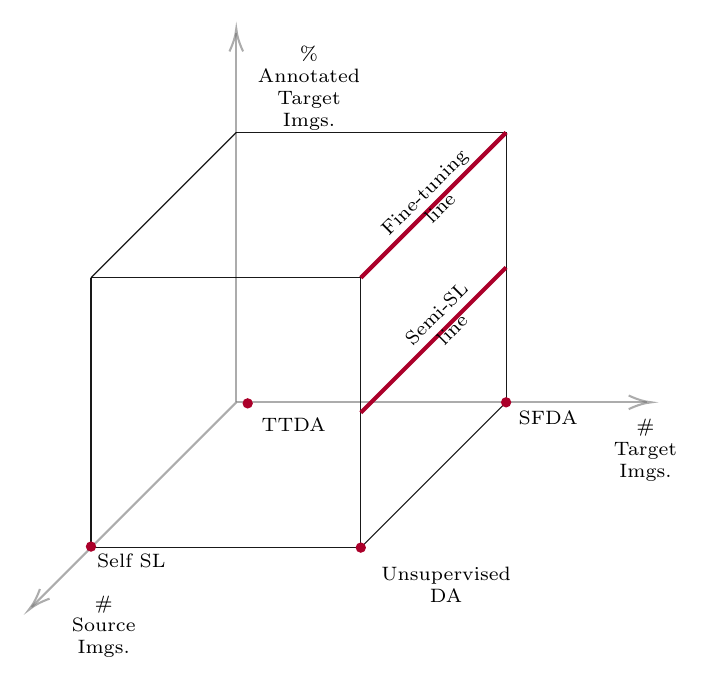
\begin{tikzpicture}[x=0.75pt,y=0.75pt,yscale=-1,xscale=1]
%uncomment if require: \path (0,402); %set diagram left start at 0, and has height of 402

%Straight Lines [id:da6807006831993536] 
\draw [color={rgb, 255:red, 117; green, 117; blue, 117 }  ,draw opacity=0.6 ][line width=0.75]    (270,210) -- (270,32) ;
\draw [shift={(270,30)}, rotate = 90] [color={rgb, 255:red, 117; green, 117; blue, 117 }  ,draw opacity=0.6 ][line width=0.75]    (10.93,-3.29) .. controls (6.95,-1.4) and (3.31,-0.3) .. (0,0) .. controls (3.31,0.3) and (6.95,1.4) .. (10.93,3.29)   ;
%Straight Lines [id:da5295149315723777] 
\draw [color={rgb, 255:red, 117; green, 117; blue, 117 }  ,draw opacity=0.6 ][line width=0.75]    (270,210) -- (468,210) ;
\draw [shift={(470,210)}, rotate = 180] [color={rgb, 255:red, 117; green, 117; blue, 117 }  ,draw opacity=0.6 ][line width=0.75]    (10.93,-3.29) .. controls (6.95,-1.4) and (3.31,-0.3) .. (0,0) .. controls (3.31,0.3) and (6.95,1.4) .. (10.93,3.29)   ;
%Straight Lines [id:da534666056608414] 
\draw [color={rgb, 255:red, 117; green, 117; blue, 117 }  ,draw opacity=0.6 ][line width=0.75]    (270,210) -- (171.41,308.59) ;
\draw [shift={(170,310)}, rotate = 315] [color={rgb, 255:red, 117; green, 117; blue, 117 }  ,draw opacity=0.6 ][line width=0.75]    (10.93,-3.29) .. controls (6.95,-1.4) and (3.31,-0.3) .. (0,0) .. controls (3.31,0.3) and (6.95,1.4) .. (10.93,3.29)   ;
%Straight Lines [id:da0025027309814475984] 
\draw [color={rgb, 255:red, 0; green, 0; blue, 0 }  ,draw opacity=0.9 ]   (270,80) -- (400,80) ;
%Straight Lines [id:da3170933147390458] 
\draw [color={rgb, 255:red, 0; green, 0; blue, 0 }  ,draw opacity=0.9 ]   (400,80) -- (400,210) ;
%Straight Lines [id:da8084774068453204] 
\draw [color={rgb, 255:red, 0; green, 0; blue, 0 }  ,draw opacity=0.9 ]   (400,210) -- (330,280) ;
%Straight Lines [id:da14868444296828032] 
\draw [color={rgb, 255:red, 0; green, 0; blue, 0 }  ,draw opacity=0.9 ]   (200,280) -- (330,280) ;
%Straight Lines [id:da9908929804494571] 
\draw [color={rgb, 255:red, 0; green, 0; blue, 0 }  ,draw opacity=0.9 ]   (330,150) -- (330,280) ;
%Straight Lines [id:da0019316496763430724] 
\draw [color={rgb, 255:red, 0; green, 0; blue, 0 }  ,draw opacity=0.9 ]   (200,150) -- (200,280) ;
%Straight Lines [id:da7518926340375516] 
\draw [color={rgb, 255:red, 0; green, 0; blue, 0 }  ,draw opacity=0.9 ]   (200,150) -- (330,150) ;
%Straight Lines [id:da3769124480681334] 
\draw [color={rgb, 255:red, 0; green, 0; blue, 0 }  ,draw opacity=0.9 ]   (270,80) -- (200,150) ;
%Straight Lines [id:da5228594606876449] 
\draw [color={rgb, 255:red, 171; green, 0; blue, 42 }  ,draw opacity=1 ][line width=1.5]    (400,145) -- (330,215) ;
%Straight Lines [id:da4767901038712239] 
\draw [color={rgb, 255:red, 171; green, 0; blue, 42 }  ,draw opacity=1 ][line width=1.5]    (400,80) -- (330,150) ;
%Shape: Circle [id:dp5300687249748464] 
\draw  [draw opacity=0][fill={rgb, 255:red, 171; green, 0; blue, 42 }  ,fill opacity=1 ] (327.5,280) .. controls (327.5,278.62) and (328.62,277.5) .. (330,277.5) .. controls (331.38,277.5) and (332.5,278.62) .. (332.5,280) .. controls (332.5,281.38) and (331.38,282.5) .. (330,282.5) .. controls (328.62,282.5) and (327.5,281.38) .. (327.5,280) -- cycle ;
%Shape: Circle [id:dp9711792189769151] 
\draw  [draw opacity=0][fill={rgb, 255:red, 171; green, 0; blue, 42 }  ,fill opacity=1 ] (273,210.5) .. controls (273,209.12) and (274.12,208) .. (275.5,208) .. controls (276.88,208) and (278,209.12) .. (278,210.5) .. controls (278,211.88) and (276.88,213) .. (275.5,213) .. controls (274.12,213) and (273,211.88) .. (273,210.5) -- cycle ;
%Shape: Circle [id:dp6127433690927064] 
\draw  [draw opacity=0][fill={rgb, 255:red, 171; green, 0; blue, 42 }  ,fill opacity=1 ] (397.5,210) .. controls (397.5,208.62) and (398.62,207.5) .. (400,207.5) .. controls (401.38,207.5) and (402.5,208.62) .. (402.5,210) .. controls (402.5,211.38) and (401.38,212.5) .. (400,212.5) .. controls (398.62,212.5) and (397.5,211.38) .. (397.5,210) -- cycle ;
%Shape: Circle [id:dp8193525877009633] 
\draw  [draw opacity=0][fill={rgb, 255:red, 171; green, 0; blue, 42 }  ,fill opacity=1 ] (197.5,279.5) .. controls (197.5,278.12) and (198.62,277) .. (200,277) .. controls (201.38,277) and (202.5,278.12) .. (202.5,279.5) .. controls (202.5,280.88) and (201.38,282) .. (200,282) .. controls (198.62,282) and (197.5,280.88) .. (197.5,279.5) -- cycle ;

% Text Node
\draw (275,37) node [anchor=north west][inner sep=0.75pt]  [font=\scriptsize] [align=left] {\begin{minipage}[lt]{43.21pt}\setlength\topsep{0pt}
\begin{center}
\% Annotated\\Target Imgs.
\end{center}

\end{minipage}};
% Text Node
\draw (447,217) node [anchor=north west][inner sep=0.75pt]  [font=\scriptsize] [align=left] {\begin{minipage}[lt]{28.38pt}\setlength\topsep{0pt}
\begin{center}
\# Target\\Imgs.
\end{center}

\end{minipage}};
% Text Node
\draw (184,302) node [anchor=north west][inner sep=0.75pt]  [font=\scriptsize] [align=left] {\begin{minipage}[lt]{31.29pt}\setlength\topsep{0pt}
\begin{center}
\# Source\\Imgs.
\end{center}

\end{minipage}};
% Text Node
\draw (331,288) node [anchor=north west][inner sep=0.75pt]  [font=\scriptsize] [align=left] {\begin{minipage}[lt]{58.26pt}\setlength\topsep{0pt}
\begin{center}
Unsupervised DA
\end{center}

\end{minipage}};
% Text Node
\draw (404.5,213) node [anchor=north west][inner sep=0.75pt]  [font=\scriptsize] [align=left] {\begin{minipage}[lt]{21.76pt}\setlength\topsep{0pt}
\begin{center}
SFDA
\end{center}

\end{minipage}};
% Text Node
\draw (342.12,185.25) node [anchor=north west][inner sep=0.75pt]  [font=\scriptsize,rotate=-315] [align=left] {\begin{minipage}[lt]{42.92pt}\setlength\topsep{0pt}
\begin{center}
Semi-SL line
\end{center}

\end{minipage}};
% Text Node
\draw (332.12,130.81) node [anchor=north west][inner sep=0.75pt]  [font=\scriptsize,rotate=-315] [align=left] {\begin{minipage}[lt]{51.53pt}\setlength\topsep{0pt}
\begin{center}
Fine-tuning line
\end{center}

\end{minipage}};
% Text Node
\draw (281,212) node [anchor=north west][inner sep=0.75pt]  [font=\scriptsize] [align=left] {\begin{minipage}[lt]{21.36pt}\setlength\topsep{0pt}
\begin{center}
TTDA
\end{center}

\end{minipage}};
% Text Node
\draw (201,282) node [anchor=north west][inner sep=0.75pt]  [font=\scriptsize] [align=left] {\begin{minipage}[lt]{25.74pt}\setlength\topsep{0pt}
\begin{center}
Self SL
\end{center}

\end{minipage}};


\end{tikzpicture}
}
\end{figure}

\Cref{fig:da_cube} depicts a conceptual model of the learning paradigms, wherein the number of unlabeled source images and labeled and unlabeled target images serve as the axes\sidenote{A representation of all the learning paradigms requires one more dimension. I had trouble representing four dimensions in a 2D paper, so I had to discard one of them.}. It can be observed that not having target labels is common, as it otherwise becomes either semi-supervised or supervised learning. Additionally, there are two scenarios that only differ in the number of target images (source-free and test-time domain adaptation) and one where no target images are available (self-supervised learning).

\begin{itemize}
    \item \textbf{Semi-Supervised DA} is very similar to traditional semi-supervised learning\sidenote{See \nameref{subsec:semi_self} in \Cref{sec:training_paradigms}.}. What defines this category is the presence of some labeled target images and a larger amount of unlabeled ones. Training strategies do not differ significantly from those used for semi-supervised learning, using the unlabeled samples for feature alignment and a regularization term that leverages the labeled samples.
    
    \item In \textbf{Unsupervised DA}, target labels are not present, and source images are often available with or without labels. This implies that the model can only learn the target domain features from feature alignment tasks, and regularization is usually done with the source images.
    
    \item \textbf{Source-Free DA} (SFDA) is a more challenging task compared to the previous two. In this setting, the model retains information about the source domain internally, but source labels and images are unavailable. This scenario is highly relevant for real-world applications where a pre-trained model is provided to a user who must fine-tune it on their unlabeled target dataset without sacrificing generalization.
    
    \item If in SFDA the model is given a whole unlabeled target dataset, \textbf{Test-Time DA} (TTDA) algorithms receive a single unlabeled sample, hence the name ``test-time''\sidenote{This is also called ``online'' training. Any other scenario with a given training set is known as ``offline'' training.}. The goal is to adapt the model parameters dynamically during the inference phase. TTDA methods often involve some kind of entropy minimization\sideauthorcite{wang2021tent} or self-training with pseudo-labels. The model is trained on each sample for a number of iterations. Therefore, each sample is evaluated using a different model, one that is tailored to the specific sample.
\end{itemize}

In \Cref{chapter:tist}, we propose a method for Unsupervised domain adaptation and evaluate it on three medical datasets. In \Cref{chapter:samda}, we use a simple test-time domain adaptation algorithm to evaluate the performance of a segmentation adapter on this task. Being the adapter a small trainable module inside a larger model---and hence its capacity very limited---we argue that it is especially suitable for tasks where the training signal is noisy, and therefore perfect for TTDA.
% Elements of Ophthalmology
%   Imaging the Retina --> technical stuff on how OCTs work and what we can get. Also fundus
%   Seeing in an OCT --> diseases that can be seen, concept of biomarker
%   Evaluating Vision: The ETDRS Grid --> Just talk about it
%   Merging DL and Ophthalmology --> How and why you would put these two together (a lot of images, difficult to segment...)

\section{Elements of Ophthalmology}
\label{sec:ophthalmology}

The methods developed in this thesis are primarily applied to ophthalmology. To provide context, we offer a concise overview of essential ophthalmological concepts that will be referenced throughout. We introduce the main retinal image modality, namely Optical Coherence Tomography (OCT), and how clinicians use it to quantify retinal thickness through the ETDRS grid. Ultimately, we demonstrate why and how deep learning can aid thousands of people when applied to ophthalmology.

\subsection{Imaging the Retina}\index{retina}\index{OCT}
The retina is located at the back of the eye, serving as the focal plane for the eye lens, as depicted in \Cref{fig:eye}. It receives the image of the visual world, and its task is to transform the incoming photons into nerve pulses. The transformation is mediated by photoreceptor cells (rods and cones) in a process that is known as \textit{visual phototransduction}. An incoming photon triggers conformational changes in the photoreceptor's membrane proteins, which begin hyperpolarization of the whole cell and, ultimately, an electrical signal\sideauthorcite{Alberts2017}. This signal travels through bipolar and ganglion cells until it finds its way through the optic nerve into the brain, where it is processed.

\textfig[t]{0.75}{Figures/retina-structure}{Light enters the eye through the cornea and projects on the retina, where rods and cones transform it into electrical impulses that travel ventrally to the optic nerve through horizontal, bipolar, amacrine and ganglion cells. Image taken from \cite{layers2016retina}}{fig:eye}

The organization of the photoreceptors and other retinal cells forms \textit{retinal layers}. Each one of these layers contains a distinct portion of the cells and is highly differentiated. Together, the layers that participate actively in the visual phototransduction receive the name of \textit{neurosensory retina} (NSR). Beyond the NSR, one layer is of special relevance because it nourishes the retinal cells: the retinal pigment epithelium (RPE). The formation of fluid pockets both inside the NSR layers or between the NSR and the RPE may have disastrous effects on visual acuity\sidedef{Visual Acuity}{Measure of the ability of the eye to distinguish shapes and the details of objects at a given distance~\cite{marsden2014measure}.}, as we will see later.

\textfig[t]{1}{Figures/interferometer.pdf}{Michelson interferometer. Low-coherence light is split into two beams. One is reflected by a mirror located at a known distance, while the other is sent to the retina and scattered back to the beam splitter, which combines their amplitudes. The detector detects an interference pattern stemming from the different path lengths the light has traveled. Reflection angles are exaggerated in this figure.}{fig:interferometer}

For years, medical imaging methods have been developed to diagnose abnormal conditions in the organism. The eye, however, might seem unexplorable at first sight due to its soft nature and its small size, ruling out more conventional methods such as X-ray or MRI. Furthermore, any technique that scans the retina must have micrometer resolution and be able to produce cross-sectional images that reveal all the retinal layers. Optical Coherence Tomography (OCT) is a non-invasive imaging technique that combines both features. Nowadays, it is used routinely in ophthalmology to scan the retina and, in particular, the region centered at the fovea. To date, it is one of the most common imaging instruments in medicine, with over 20 million OCT scans taken each year worldwide\sideauthorcite{fujimoto2016development}.

OCT uses low-coherence interferometry. As illustrated in \Cref{fig:interferometer}, infrared light is split into two beams. One is reflected by a mirror located at a known distance, while the other is sent to the retina and scattered back to the beam splitter, which combines their amplitudes. The combined wave produces an interference pattern at the detector. This is measured to infer the properties of the retina at the scanning point. By shifting the scanning point, one can acquire a B-scan, \ie~a 2D cross-sectional image of the retina, as depicted in \Cref{fig:oct_scans} (left). A stack of ordered B-scans is known as a C-scan, \ie~a 3D representation of the retina, as shown in \Cref{fig:oct_scans} (right).

\textfig[t]{1}{Figures/oct_scans.pdf}{(Left) 2D cross-sectional image of the retina, also known as B-scan. (Right) 3D representation of the retina, or C-scan. Image partially reproduced from~\cite{Kurmann2019}}{fig:oct_scans}

\subsection{Seeing in an OCT}\index{biological marker}\index{intraretinal fluid}\index{subretinal fluid}
OCT provides a cross-sectional view of the retina. It displays all the retinal layers with different shades of gray that depend on the layer's reflectivity\sidenote{See the retinal layers in \Cref{fig:oct_scans} as horizontal lines with different shades of gray.}. For this reason, it is the preferred imaging technique to evaluate the retinal morphology, such as its thickness or the presence of fluid\sidenote{In fact, the presence of fluid increases the retinal thickness; both properties are correlated.}. Abnormal values of these properties are directly linked to potentially disastrous eye conditions, and they are called \textit{biological markers}\sidedef{Biological Marker}{Objective indications of medical state observed from outside the patient – which can be measured accurately and reproducibly~\cite{strimbu2010biomarkers}.} --- or biomarkers--- for this reason. 

The presence of fluid is of special relevance to this thesis, with \Cref{chapter:oct} diving into the methods to localize fluid pockets from OCT B-scans. More specifically, we will be interested in intraretinal and subretinal fluid (IRF and SRF, respectively):
\begin{itemize}
    \item \textbf{Intraretinal fluid (IRF)} is identified as hypo-reflective areas in the NSR layers, usually above the outer plexiform layer\sidecitation{haines2017fundamental}{The outer plexiform layer contains synapses among and between retinal photoreceptors, horizontal cells, and bipolar cells.}. It is associated with decreased visual acuity\sideauthorcite{sharma2021understanding}.

    \item \textbf{Subretinal fluid (SRF)} also appears as hypo-reflective areas in the OCT, but it is located beneath the NSR and above the RPE. The studies suggest, however, that a mild amount of SRF may be tolerated or even beneficial in terms of visual acuity\sideauthorcite{chaudhary2022association}.  
\end{itemize}

Both biological markers are associated with pathologies such as Age-Related Macular Degeneration (AMD) or Diabetic Retinopathy (DR). These pathologies affect the capillaries that nourish the retina. If they are not treated adequately, they may lead to fluid loss in the form of fluid pockets.

\subsection{Evaluating Vision: The ETDRS Grid}\index{ETDRS grid}
The quantification of the retinal morphology is only one step into the vision evaluation through OCT. Analyzing thickness data is complex, as every point of each retinal layer has one thickness value. While this enables a spatially precise evaluation of the layers, it is more meaningful in clinical practice to summarize thickness changes in larger retinal areas, effectively reducing the amount of data to analyze. Established methods for summarizing retinal thickness data utilize retinal grids centered in the macula to divide the retina into large regions of interest. These grids allow for the aggregation of thickness measurements for each region, providing a quick overview of the layers' thickness in anatomically predefined areas. 

The most common grid type for retinal thickness aggregation was introduced by the Early Treatment Diabetic Retinopathy Study (ETDRS)\sideauthorcite{early1991grading} and is known as the ETDRS grid. It divides the retina into nine regions defined by three rings centered around the fovea: a \qty{1}{\milli\metre}-diameter central ring, an inner macular ring with \qty{3}{\milli\metre} diameter, and an outer macular ring with \qty{6}{\milli\metre} diameter. Furthermore, the 3 and \qty{6}{\milli\metre} rings are divided into four quadrants: nasal, temporal, superior, and inferior. The retinal thickness is averaged for all the points in a region so that only one value is stored. Figure \Cref{fig:etdrs}, from \yeartextcite{rohlig2019enhanced}, illustrates the ETDRS grid in a coronal plane located at the retina (a and b), and in a transverse plane that passes through the fovea (c and d). 

\textfig[t]{1}{Figures/etdrs.png}{ETDRS grid. (a, b) It divides the retina into nine regions defined by three rings centered around the fovea. (c) A B-scan with an overlain ETDRS grid. (d) Layer thickness quantification. Figure from \cite{rohlig2019enhanced}.}{fig:etdrs}

The aggregation of thickness data in predefined regions facilitates the tracking of progressive diseases while considering the natural variations of the retina. This aspect has been crucial for the rapid spread of the ETDRS grid for disease assessment, as the different ETDRS ring regions are linked to different visual function levels. 

\subsection{Merging Deep Learning and Ophthalmology}
Early diagnosis and treatment of ocular diseases are key to slowing down the progress of symptoms, and OCT is the preferred diagnostic tool to image the retina due to its safety and quickness. However, every year, around 30 million OCT retinal scans are acquired and processed, and clinics are running out of experts to interpret them. These experts use biological markers to assess the presence of several conditions. Still, the variety in shape, size, and extent of said markers makes even their coarse location a paramount task. On the other hand, deep learning models are becoming faster and more capable, showing on-par performance compared to humans in some tasks\jgt{cite}. The marriage of both worlds seems, therefore, inevitable. 

Nevertheless, the introduction of AI methods into a medical field, such as ophthalmology, must be done carefully and respectfully. Several methods have been proposed in recent years that see the problem only from one side\sidenote{Usually, that side is computer science.}  and therefore lack the general view that clinicians have acquired over years of practice, errors, and successes. This is the case of \yeartextcite{gulshan2016development}, a work that compared an automated deep learning algorithm against manual grading by ophthalmologists for diabetic retinopathy in retinal fundus photographs\sidedef{Retinal Fundus Photograph}{Medical image captured of the interior surface of the eye, including the retina, optic disc, and macula.}. After achieving promising results on diabetic retinopathy datasets, the system received official medical device certification and was deployed in India and Thailand\sideauthorcite{google2019retina}. Despite the previous encouraging results, the system faced significant challenges in deployment, mainly due to data quality\sideauthorcite{widner2023lessons}.
